\subsubsection{INA226}

El \texttt{INA226} es un sensor de corriente y tensión que reporta las medidas a través de \texttt{I²C}. En el sistema se utilizan para medir tanto la tensión como la corriente del panel solar, la batería de backup y las baterías a cargar (\texttt{BAT1} y \texttt{BAT2}).\cite{texasinstrumentsINA22636V16Bit}

\begin{figure}[h]
    \centering
    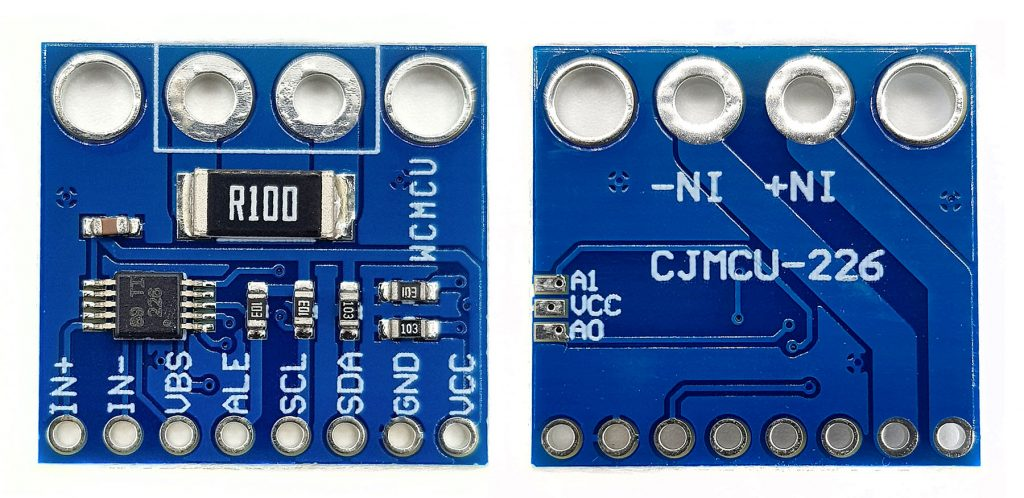
\includegraphics[width=0.5\textwidth]{images/2-hardware/componentes/INA226.jpg}
    \caption{\texttt{INA226}}
    \label{fig:hardware/modulos/ina226}
\end{figure}

Para poder medir de forma precisa, se utiliza un resistor \texttt{shunt}, una resistencia con valor muy bajo que se coloca en serie con la carga para medir la corriente que circula por ella. La tensión que cae en el resistor \texttt{shunt} es proporcional a la corriente que circula por él, y el \texttt{INA226} mide esta tensión para calcular la corriente que circula por el circuito.

La dirección \texttt{I²C} del sensor se puede configurar mediante los terminales \texttt{A0} y \texttt{A1}, uniendo estos a \texttt{VCC}, \texttt{GND}, \texttt{SDA} o \texttt{SCL}. En nuestro caso, se ha configurado la dirección \texttt{I²C} de la siguiente forma:

\begin{itemize}
    \item \texttt{INA226} del panel solar: \texttt{0x45}
    \item \texttt{INA226} de la batería de backup: \texttt{0x40}
    \item \texttt{INA226} de la batería \texttt{BAT1}: \texttt{0x44}
    \item \texttt{INA226} de la batería \texttt{BAT2}: \texttt{0x41}
\end{itemize}

\begin{figure}[h]
    \centering
    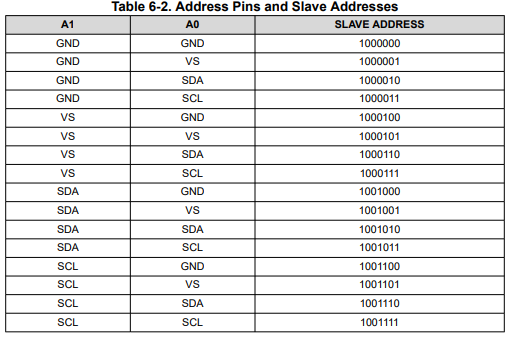
\includegraphics[width=0.7\textwidth]{images/2-hardware/componentes/direcciones_ina.png}
    \caption{Posibles direcciones \texttt{I²C} del \texttt{INA226}}
    \label{fig:hardware/modulos/direcciones_ina}
\end{figure}